\documentclass{article}
\usepackage{graphicx} % Required for inserting images
\usepackage{amsmath}
\usepackage{amssymb}
\usepackage{amsthm}
\setlength{\parindent}{0pt}
\usepackage[dvipsnames]{xcolor}
\newcommand{\lra}{\ensuremath\longrightarrow}
\usepackage{caption}
\usepackage{subcaption}
\usepackage[section]{placeins}
\usepackage{tabularx}
\usepackage{hyperref}
\hypersetup{
    colorlinks=true,
    linkcolor=cyan,
    filecolor=magenta,      
    urlcolor=blue,
    citecolor=black,
    pdfpagemode=FullScreen,
    }
\usepackage{matlab-prettifier}
\usepackage[
  backend=biber,
  citestyle=numeric,
  autocite=superscript,
  bibstyle=authortitle
]{biblatex}
\addbibresource{bibliography.bib} 

\usepackage[margin=1in]{geometry}

\title{Final Project 4320}
\author{Brookes HeilBlackburn, Justin Raimundo}
\date{April 2025}

\begin{document}

\maketitle

\section*{Introduction}
Given recent events in our community we were motivated to understand how scientists model wildfires.  We were hopeful to see how our first semester partial differential equations material might be useful to scientists who do research that helps people prepare, control and/or mitigate wild fire impacts.\\\\
The first section begins with our initial exploration into wildfire models.  The second section discusses why we felt it was important to analyze complex real world models with numerical methods followed by what we learned in using those methods.  We conclude with a summary of what we learned in the process of using basic numerical methods.

\section*{Wildfire Model Exploration - Types of Models}
\section{Models}
In this section of our paper we will share 3 of the wildfire models we read.  These span roughly the level of complexity that we encountered.  We begin by walking through the simplest of models that is based on a traveling wave epidemiological model.  Followed by reviewing a piece of the highly complex multi-layered family of models that are used in real world environments for modeling rate of fire spread.  We wrap up with a model that is friendly to mathematicians.  This will lead us to conclude our discussion on models and why we decided to explore numerical methods.
\subsection{Logan\supercite{logan} Epidemic Wave}
We were advised that we might consider the similarities between the epidemic wave model found in Logan Chapter 5 section 2 with how a wildfire might behave\supercite{logan}.  The 2-equation system is a basic version of the SI model (Susceptible, Infectious).  Quite quickly we found the conceptual substitution seen in the figure below.
\begin{center}
    {\large  Susceptible-Infected Model:\\
    $\textcolor{MidnightBlue}{S_t} = -\textcolor{magenta}{b}SI$\qquad
    $\textcolor{MidnightBlue}{I_t} = \textcolor{magenta}{b}SI-\textcolor{red}{r}I+\textcolor{orange}{D}u_{xx}$}\\
    \begin{minipage}[t]{.49\textwidth}
    \centering
    SI/fire Function - MATLAB    
    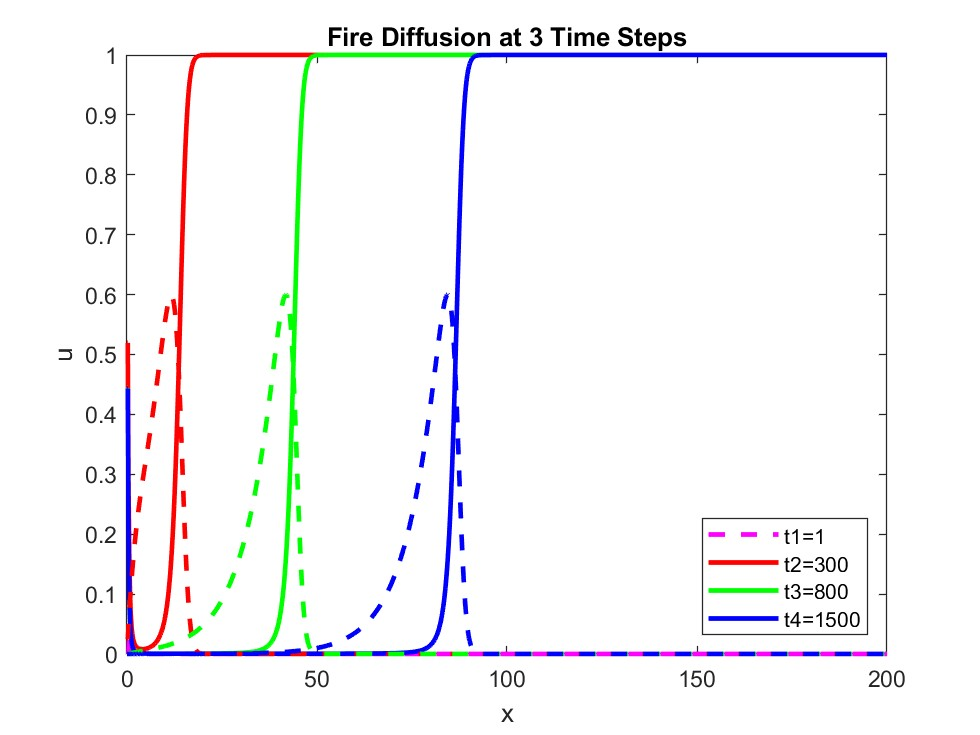
\includegraphics[scale=0.17]{Step1_HS_Gaussian_Advection_Diffusion_3_timestamps.jpg}
    \end{minipage}
    %
    \hfill
    \begin{minipage}[t]{.49\textwidth}
    \centering
    SI Function Logan Book    
    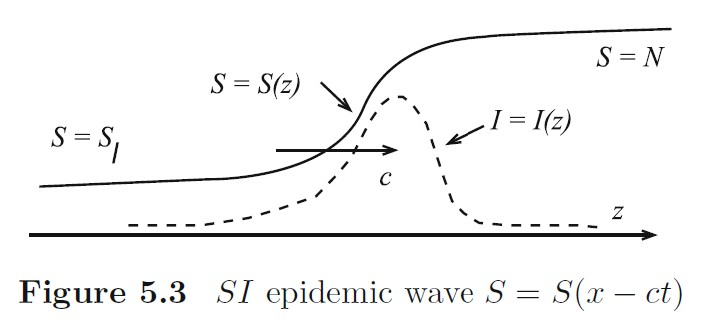
\includegraphics[scale=0.5]{1D_epidemic_from_book.jpg}
    \end{minipage}\\  
    $\textcolor{MidnightBlue}{S_t=}\text{Susceptible,}\quad\textcolor{magenta}{b=}\text{Infection Rate,}\qquad
    \textcolor{MidnightBlue}{I_t=} \text{Infected,}\quad\textcolor{orange}{D=}\text{Diffusion Rate}$\\
    $\textcolor{MidnightBlue}{S_t=}\text{Healthy Trees,}\quad\textcolor{magenta}{b=}\text{Burn Rate,}\qquad\textcolor{MidnightBlue}{I_t=} \text{Burning,}\quad\textcolor{orange}{D=}\text{Spread Rate}$
\end{center}
The image on the right was taken from the Logan textbook.  It shows 2 stable states with an abrupt point of perturbation. 
The image on the left is a graph we were able to generate in MATLAB \textit{after} having learned basic numerical methods and applying them to the SIR equations in Logan.  At face value the conceptual variable substitution while potentially valid did not provide useful intuitive understanding of the mechanics of either of the processes modeled. It was through the studying and creation of the image on the left that we began to scratch the surface of the math in the SIR model. Through this course of study we started to understand the value of numerical methods.
\subsection{Rothermel Model}
Patricia Andrews\supercite{andrews} published an approachable, comprehensive compilation of inputs and outputs of the evolving fire models using Rothermel's\supercite{rothermel} surface fire spread model. \\
In her work "The Rothermel Surface Fire Spread Model and Associated Developments: A Comprehensive Explanation", she reminds us of the idea developed in Sullivan's\supercite{sullivan} work in 2009\cite{sullivan} that classified and categorized fire models. The Rothermel fuel spread model fits into the category of a quasi-empirical model.  It is based in physics and chemistry equations and further refined with empirical data observations. The model has been refined over time by various researchers. The basic single-dead-fuel type model is based on prior work in fire modeling developed around the conservation of energy principle. Subsequent models were created based on Rothermel's work. The basic surface spread fire model is a series of equations that results in a rate of spread given by:
$$R=\frac{I_R\xi(1+\phi_w+\phi_s)}{\rho_b\xi Q_{ig}}$$
$R=$ rate of spread at the flaming front\\
$I_R=$ reaction intensity as energy release per unit area\\
$\xi=$ Propogating flux ratio (proportion of adjacent particles that ignite)\\
$\phi_w=$ wind factor\\
$\phi_s=$ slope factor\\
$\rho_b=$ bulk density - oven dry fuel per cubic foot\\
$Q_{ig}=$ heat of preignition - heat require to ignite 1 pound of fuel\\
The early forms of the model required data and physical principles.  Each term in the above is derived from experimental data, physical and mathematical principles.  The model was later adapted with weighting factors for use in the field applications.\\

\begin{minipage}{.47\textwidth}
        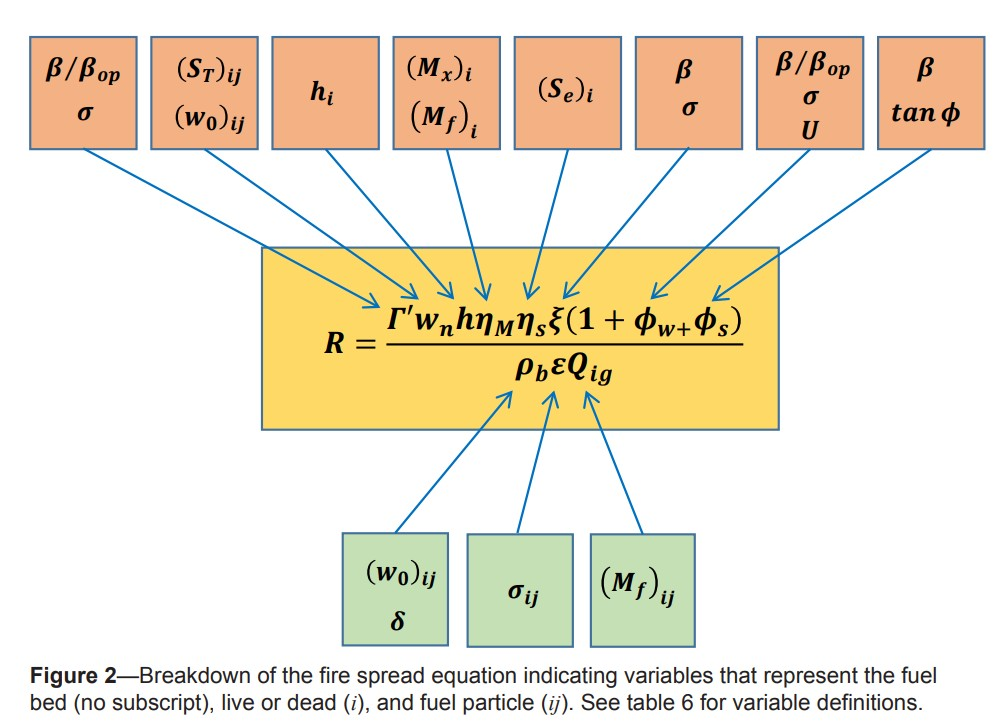
\includegraphics[scale=0.35]{Andrews_final_spread_equation.jpg}
\end{minipage}
%
\hfill
%
\begin{minipage}{.47\textwidth}
    $\frac{\beta}{\beta_{op}}=$ Relative packing ratio\\
    $s$ variables related to mineral content\\
    $h_i$ heat content\\
    $M$ variables related to moisture content\\
    $tan\phi$ slope steepness\\
    $w$ fuel load\\
    $\sigma$ surface area to volume ratio
\end{minipage}\\
\\
Andrews discusses how the weighting for each of the different parameters is derived. A large portion of the remainder of the paper expands on adjustments to subsystems that calculate fuel.  There is discussion of software tools that are based on Rothermel's surface spread methods in tools used to this day.
$$\phi_E=\phi_w+\phi_S \quad \text{Effective Wind Speed}$$
$$t_r=8d\quad \text{Residence Time}$$
$$H_A=I_Rt_r\quad \text{Heat per Unit Area}$$
$$I_B=HwR\quad \text{Fireline Intensity}$$
$$F_B=0.451_B^{0.46}\quad \text{Flame Length}$$

There is further discussion on the importance of the subsystem for modeling fuel characteristics described as standard, dynamic, custom, and special case fuel models. Each of which is a complex model of its own. This multi-layered systems within systems developed over decades while practically more realistic is beyond our abilities in our current level of study.  We continued our search for a simplified fire model.  

%----------------Idealized Math Model
\subsection{Idealized Forest Fire Model}
In a 2009 article for the SIAM Journal on Applied Mathematics Babak, Bourlioux and Hillen\supercite{babak} wrote about the effects of wind in a 1D traveling wave model for an idealized forest fire scenario.  Their model is an advection-reaction-diffusion system.  While it makes assumptions that are unrealistic, it allows them to isolate and analyze wind advection forces at the fire front. Reviewing this idealized model we began to relate the complicated Rothermel based systems with the simplified SIR summary.   Unlike Rothermel and subsequent field models, this analysis is purely a mathermatical exercise. They start with physics and chemistry based equations for combustion and reaction respectively. \\\\
\textbf{2D Combustion (Physics):}
    $$\rho C\left(\frac{\partial T}{\partial t}+\vec{w}\cdot \nabla T\right)=k\Delta T +\rho Q \cdot R(T,|w|)Y$$
    $$\frac{\partial Y}{\partial t}=-R(T,|w|)Y$$
The basic form is similar to what we see in the diffusion equations thus far.  The left hand side showing us a change in temperature with respect to time.  The right hand side a diffusion element and a reaction term.  
The basic heat equation:
$$u_t=\alpha u_{xx}$$
where $\alpha = \frac{k}{\rho C}$.  If we divide both sides by $\rho C$ we see $\alpha$ on the right hand side multipled by the second spatial derivative.   Depending on if the reaction we will have either a source or sink function.  The second equation calculates the change in fuel with respect to time.\\
\textbf{Arrhenius Reaction Equation (Chemistry):}
    $$R(T,|w|) =Ae^{-\frac{E}{\hat{R}RT}}\mathcal{H}(T-T_{ig}).$$ 
    $T(t,x)\text{ temperature }\&\, Y(t,x)\text{ fuel mass fraction}$; 
    $|w|=\text{wind velocity},$; 
    $\rho \text{= density of fuel}(kg\cdot m^{-3})$; 
    $C=\text{specific heat of fuel }(J\cdot kg^{-1}\cdot K^{-1}),$;  $k=\text{ thermal conductivity of fuel }(J\cdot s^{-1}m^{-1}K^{-1}),$; 
    $Q=\text{ heat of combustion }(J\cdot kg^{-1})$; 
    $T_{ig}$ fuel must reach this to combust; 
    $R(T)=$ reaction rate; $E\ (J\cdot mol^{-1})=$ activation energy; $\hat{R}(8.314J\cdot mol^{-1}K^{-1})$ universal gas constant.  $\mathcal{H}(z)=$ heaviside step function. \\
    Through non-dimensionalization 
    $$\tilde{x}=\frac{x}{L},\quad \tilde{t}=\frac{k}{\rho C L^2},\quad \vec{\tilde{w}}=\frac{\rho C L}{k}\vec{w},\quad \tilde{u}=\frac{C}{QY_\infty}(T-T_\infty),\quad \tilde{v}=\frac{Y}{Y_\infty},$$
    they arrive at
    $$\frac{\partial u}{\partial t}+\vec{w}\cdot \nabla u=\Delta u + r(u,|w|)v,\quad \frac{\partial v}{\partial t}=-r(u,|w|)v,$$
    where
    $$r(u,|w|)=\frac{\rho C L^2}{k}\vec{w}R \left(u\frac{QY_\infty}{C}+T_\infty, \frac{k}{\rho C L}|w|\right)$$
    with $T_\infty$ and $Y_\infty$ representing ambient conditions for temperature and fuel respectively.  Through key assumptions, boundary conditions and traveling wave set up, the resulting system can be understood through the lens of what we have learned in our first semester partial differential equations class.  \\
    Key assumptions include:
    $$\theta=\frac{C}{QY_\infty}(T_{ig}-T_\infty)\quad (\text{ignition point at: }\eta=0) \quad \eta = x_1-ct$$
    Ahead of the front(unburned region) at $\eta=+\infty$ the Boundary Conditions are: 
    $$\theta<0 \quad u(+\infty)=0, \quad v(+\infty)=1\quad v(\eta)=1 \quad \eta>0$$
    In the above, ingition value $\theta$ has not been reached. Nothing has burned $u(+\infty)$, also represented by the fuel is unburned $v(+\infty)$ \\
    Behind the front $\eta=-\infty$ the Boundary Conditions are:
    $$u(-\infty)=1, \quad v(-\infty)=0\qquad u(0)=\theta\quad$$
    The ignition happened at $\eta=0$ and everything is now burned.\\
    This results in a now familiar differentiated and rewritten system with respect to $\eta$
    $$(w-c)u'=u''+r(u,|w|)v,$$
    $$-cv'=-r(u,|w|)v,$$
After reviewing several models, including the 3 here, we found that we still wanted to understand more. Throughout our research, explanations and understanding of data were primarily understood with numerical methods. We continued on with reviewing these models with numerical methods.

\section{Basic Numerical Methods}
Logan provided a 1D wave graphic that reflected the epidemic model. We had yet to understand the behavior and contributions of the elements of the equations that generated these graphics.
We were hopeful that we could glean insights into how researchers use numerical methods. It was surprising the relative ease with which we were able to quickly see the benefit of numerical implementations of math models.

 To begin studying numerical methods we took note of the first and second partial derivatives in both models. They each have a diffusion structure. Starting simple with advection we proceed to code diffusion and a combination of advection and diffusion.  This section concludes with a review of coding the Susceptible-Infectious model. 
\subsection{Finite Difference Method}
The finite difference method is a numerical method for estimating a derivative in discretized environments.  First and Second Derivatives can both be estimated.  We look at the former with an explicit method, and the latter with both explicit \& implicit methods. This section includes a discussion on the sensitivity of the models, boundary conditions and wraps up with an SI model discussion.   \\
As we are taught in Calculus I the formula for a derivative analytically is:
$$f'=\lim_{h\rightarrow0}\frac{f(x+h)-f(x)}{h}$$
Which can be written in Taylor expansion as:
$$f(x+k)=f(x)+\frac{f'(x)\cdot k}{1!}+\frac{f''(x)\cdot k}{2!}+\dots +\mathcal{O}(k^{n+1}) $$
This is a very helpful representation when trying to implement into a numerical system on a computer. Logan does a careful derivation explanation that arrives at the explicit forward difference approximation for the partial derivatives $u_x\,\& \,u_t$:
$$u_x(x,t)=\frac{u(x+h,t)-u(x,t)}{h}+\mathcal{O}(h)$$
and
$$u_t(x,t)=\frac{u(x,t+k)-u(x,t)}{k}+\mathcal{O}(h)$$
where $\mathcal{O}(k^{n+1})$ is an error term.  The similarities to the analytic derivative are noted.  This is the explicit form of calculation. In other words, the next element in the calculation is based solely on prior steps.  Later in this section we will discuss the implicit method where future solution steps require future estimated values.\\
Once programmed in MATLAB, we could manipulate these equations to gain better insights into their behavior.  \\
\subsection{Advection - Explicit $1^{st}$ Partial Derivative}
Starting simply we use a forward difference method on a basic advection equation.  We will be using $u_t$ to represent the about of fuel burned with respect to time.
$$u_t=cu_x$$
\\
    \begin{minipage}[t]{.49\textwidth}
        \centering
            Heaviside Steady State Transition
            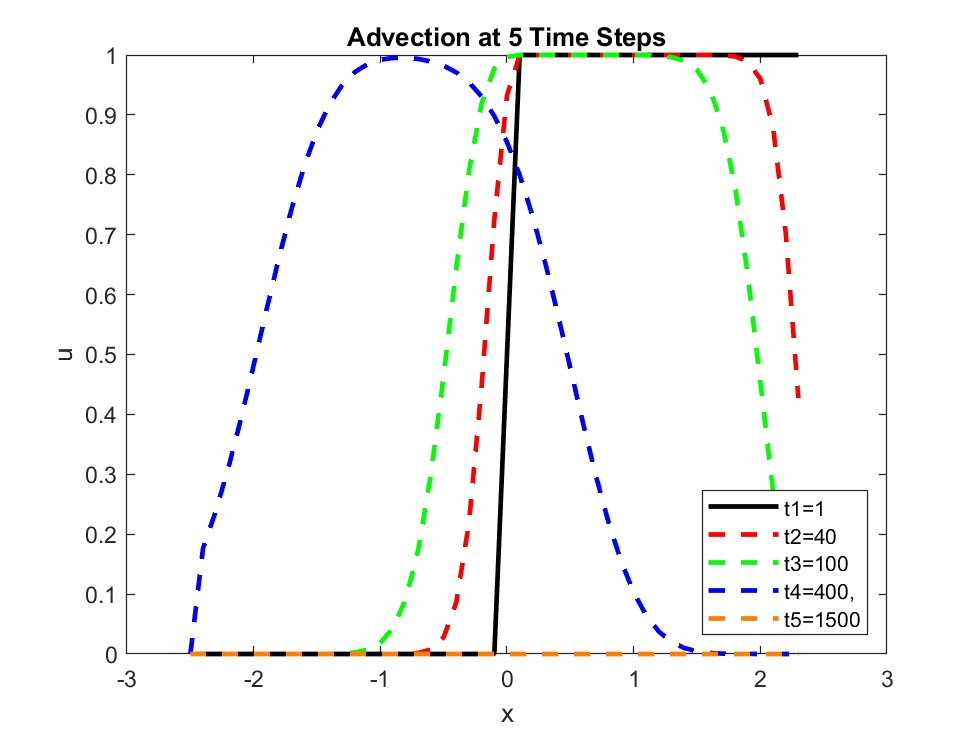
\includegraphics[scale=0.20]{Step1_HS_Advection_5_timestamps.jpg}
            \captionof{figure}{\small{Basic Advection with Heaviside Function}}
            \label{fig:HS-Advection}
    \end{minipage}
    \hfill
    \begin{minipage}[t]{.49\textwidth}
        \centering
        Heaviside Hat Function
       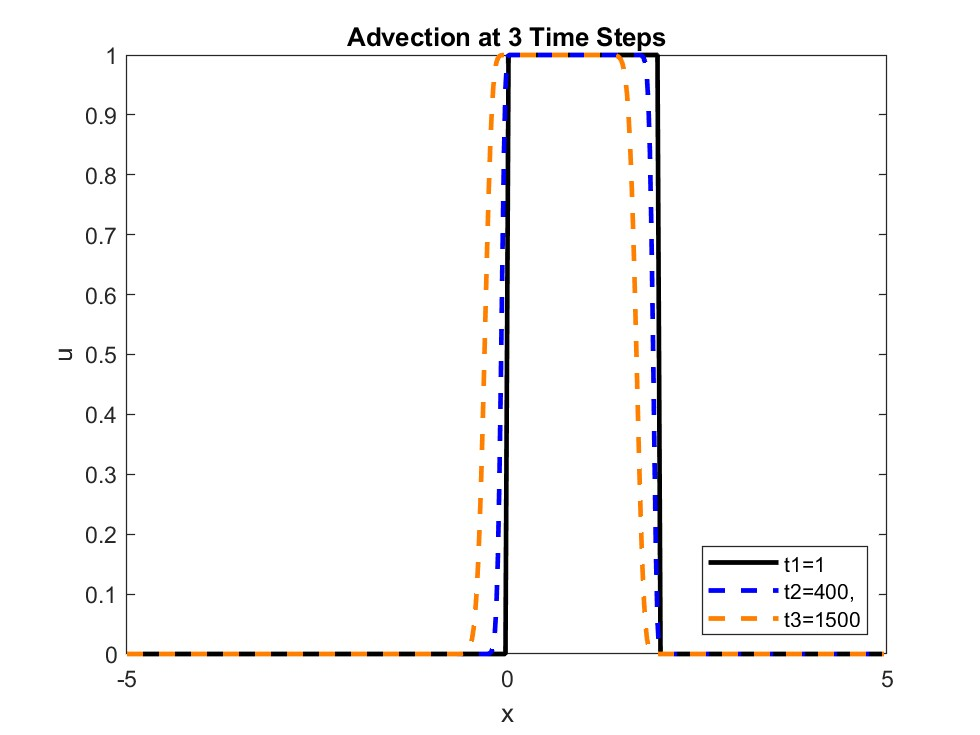
\includegraphics[scale=0.20]{Step1_Hat_Advection_3_timestamps.jpg}
       \captionof{figure}{\small{Basic Advection with Hat Function}}
       \label{fig:Hat-Advection}
    \end{minipage}
    \vspace{.5cm}
In the left-hand graph we see that this basic advection model at $t_0$ shows a quick state change from state 0 to state 1.  This graph is useful in reading a spatial dimension on the horizontal axis.    The left-hand graphic is problematic when considered in the fire modeling perspective. This shows that trees "to the right" of space 0 are state 1 (healthy) and "to the left" are state 0 (burned). The advection wave should visually move one direction.  In our case, left.  Material to the left of 0 will enter the burn region and material to the right should be spared as the advection is moving away from that region.  However what we are seeing is that things to the right of space 0 at later timesteps are burning even though the propagation wave is moving away from it.  This would not be expected in fire behavior solely under advection forces. \\
The graph on the right shows us the expected behavior of an advection traveling wave. There is a constant function shape that shifts in the direction of the propagation wave. 
\subsection{Heat/Diffusion Equation- Explicit $2^{nd}$ Partial Derivative}
The next step was to look at a slightly more complicated equation that involved a second derivative, The Diffusion Equation:
    $$u_t=Du_{xx}$$
We began with an explicit form of diffusion that required understanding of stability in implementing partial differential equations in computers.  The second derivative in the forward difference method can be described by:
    $$\frac{U_j^{n+1}-U_j^n}{k}=D\left(\frac{U^n_{j-1}-2U_j^n+U_{j+1}^n}{h^2}\right)$$
with $x_j=jh$ and $t_n=nk$ and:
    $$r=\frac{kD}{h^2}$$
resulting in:
    $$U_j^{n+1}-U_j^n=r(U^n_{j-1}-2U_j^n+U_{j+1}^n)$$
It is noted that if the time step is too large the calculation can become inaccurate/unstable resulting in erroneous information.  In Logan we are advised of a basic stability condition of $r\leq \frac{1}{2}$.  In our implementation in MATLAB we set $k=\frac{h^2}{D}$.  This proved to be stable enough for this basic representation of the diffusion equation.\\
    \begin{minipage}[t]{.49\textwidth}
    \centering
    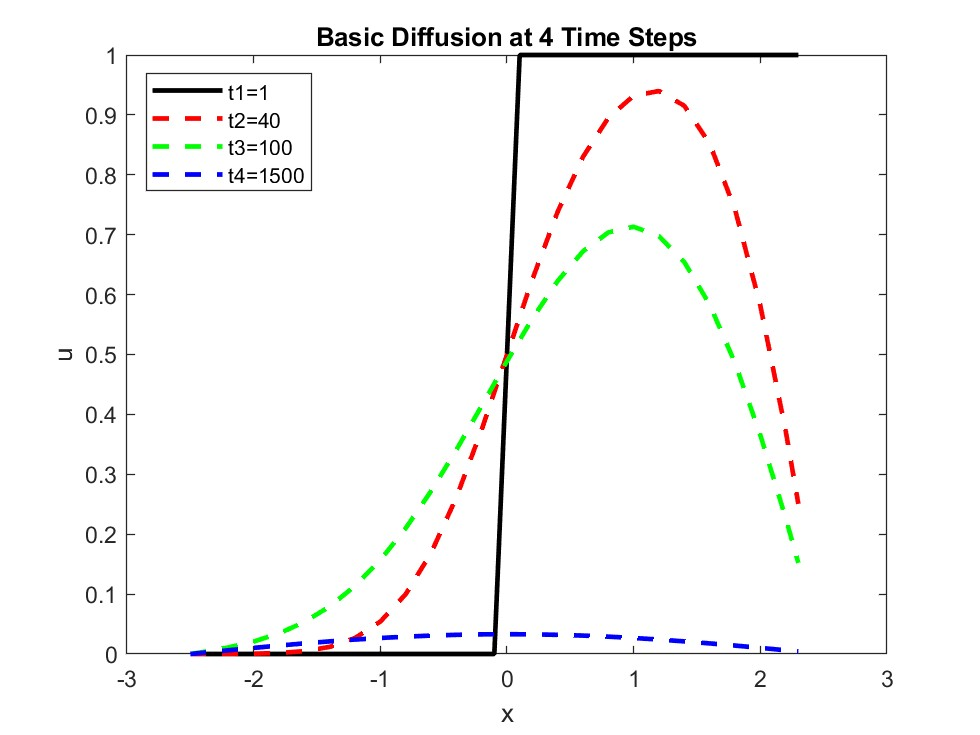
\includegraphics[scale=0.20]{Step1_HS_Diffusion_4_timestamps.jpg}
    \captionof{figure}{\small{Basic Diffusion with HS Function}}
    \label{fig:HS-Diffusion}
    \end{minipage}
    \hfill
    \begin{minipage}[t]{.49\textwidth}
    \centering
    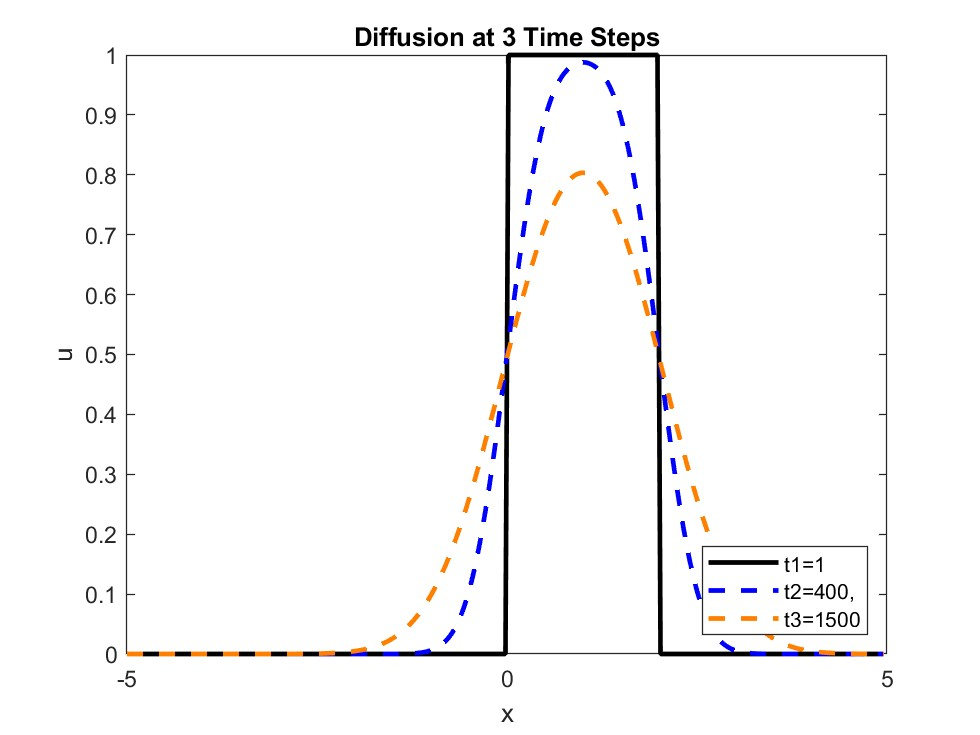
\includegraphics[scale=0.20]{Step1_Hat_Diffusion_3_timestamps.jpg}
    \captionof{figure}{\small{Basic Diffusion with Hat Function}}
    \label{fig:Hat-Diffusion}
    \end{minipage}
\vspace{.5cm}

Similar to advection, we see the unexpected behavior in the left graph.  The right graph gave an immediately intuitive visual of how one would expect material to diffuse out from the center of a location.\\
\subsection{Dirichlet Boundary Condition}
At this point we wanted to analyze the erroneous behavior we were seeing on the left graphs in both advection and diffusion.  At this point we began to understand the symbiotic nature of the model to the math and vice versa.  Through trial and error we found that setting the boundary conditions at $+\infty=1$ we would see the behavior of a state transition we would expect. This led to a deeper understanding of what Dirichlet boundary conditions are and how they impact a model.  It also later helped us understand why the SIR model in Logan behaved differently at the one end of the spatial domain.\\
    \begin{minipage}[t]{.49\textwidth}
    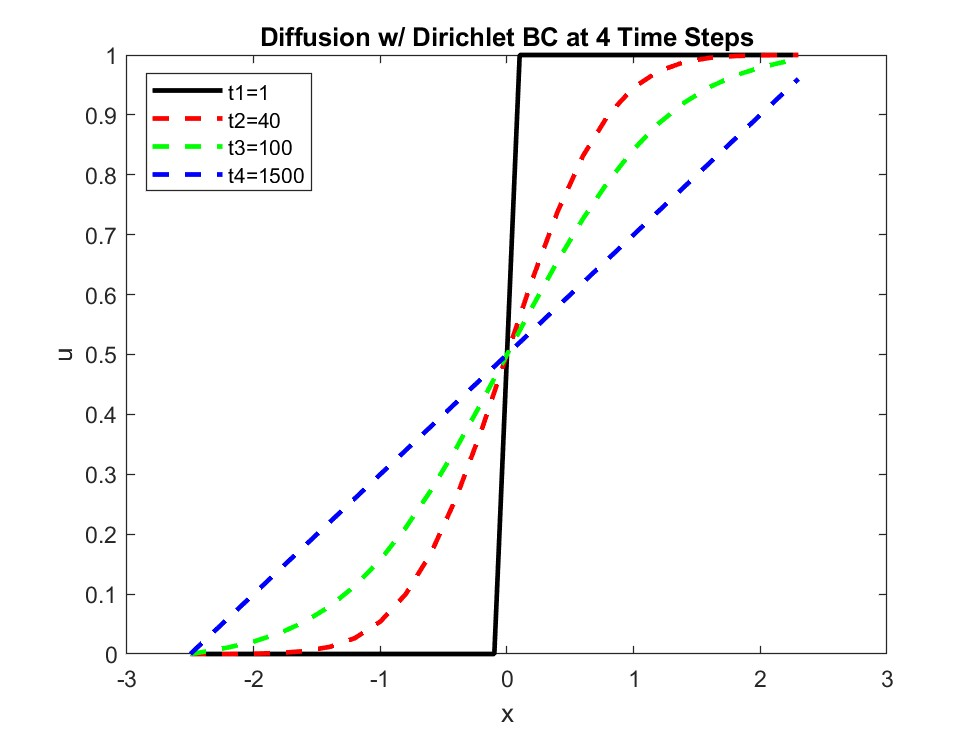
\includegraphics[scale=0.20]{Step1a_HS_Diffusion_Dirichlet_4_timestamps.jpg}
    \captionof{figure}{\small{Direchlet Diffusion with HS Function}}
    \label{fig:HS-Dirichlet-Diffusion}
    \end{minipage}
    %
    \hfill
    %
    \begin{minipage}[t]{.49\textwidth}
     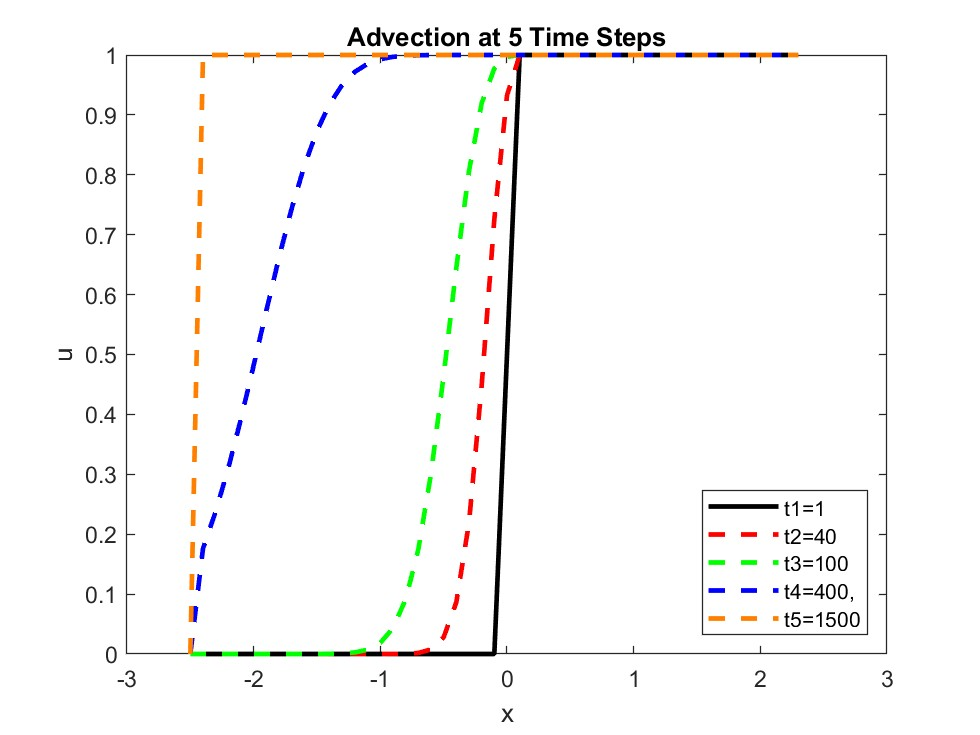
\includegraphics[scale=0.20]{HS_Advection_Dirichlet_5_timestamp.jpg}
     \captionof{figure}{\small{Dirichlet Advection with HS Function}}
    \label{fig:HS-Dirichlet-Advection}
    \end{minipage}
\vspace{.5cm}

The graph on the right helped us more deeply understand the spatial horizontal axis and the time step curves.  Most unique was at $t_5=1500$. Through writing the code and manipulating the parameters we interpreted the orange dashed line to represent the region to the left of $\eta=0$ that would burn some time later than the point of origin.  The abrupt transition at the boundary being the result of the interval defined in MATLAB.  The graph on the left was not yet as helpful as we still work to understand what it is telling us.  It appears to mean that at the later time steps there will be a final stable linear relationship across the spatial domain.  We moved onto the next step of exploration where we combined what we had learned thus far.
\subsection{Combined Advection-Diffusion Model - Explicit and Implicit}
Our goal was to be able to setup the SI model as visualized in Logan.  We had surmised that we would need both advection and diffusion in that model so we worked to combine the two.
\\
This system led to instabilities that were not readily overcome with the methods we had learned thus far.  This required further research into ensuring stability in numerical methods.  We implemented the implicit difference method as described in Logan\supercite{logan} and Bradie\supercite{bradie} for the diffusion portion of the system. In this process the next time step is found by solving a linear system of equations that are set equal to an algebraically rearranged weighted average of the next and current time step. We used the Crank-Nicolson scheme that sets the weighting factor $\theta=\frac{1}{2}$. It is a more stable numerical process that is not as sensitive to the size of the timestep. Represented here:\\
$$\frac{U_j^{n+1}-U_j^n}{k}=D\theta\left(\frac{U^{n+1}_{j-1}-2U_j^{n+1}+U_{j+1}^{n+1}}{h^2}\right)+D(1-\theta)\left(\frac{U^n_{j-1}-2U_j^n+U_{j+1}^n}{h^2}\right)$$
with $x_j=jh$ and $t_n=nk$ and:
$$r=\frac{kD}{h^2}$$
Rearranges to become:
$$-\theta r U_{j-1}^{n+1}+(1+2r\theta)U_j^{n+1}-\theta rU_{j+1}^{n+1}=(1-\theta)rU_{j-1}^n+[1-2(1-\theta]U_j^n+(1-\theta)rU_{j+1}^n$$

\begin{center}
    \begin{minipage}[t]{.49\textwidth}
    \centering
    {\Large Advection Diffusion Formula: $\textcolor{MidnightBlue}{u_t} = \textcolor{orange}{D}u_{xx}-\textcolor{magenta}{c}u_{x}$}
    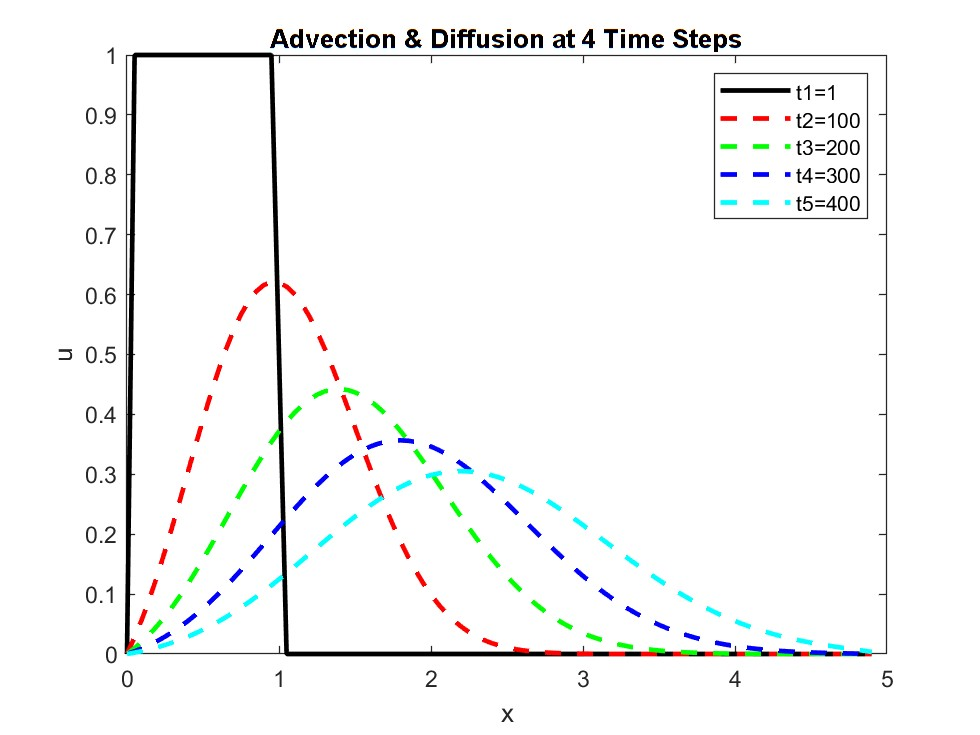
\includegraphics[scale=0.20]{Hat_Advection_Diffusion_4_timestamp.jpg}
    \captionof{figure}{\small{Advection and Diffusion Combined}}
    \label{fig:Advection-Diffusion}
    \end{minipage}
    %
    \hfill
    %
    \begin{minipage}[t]{.49\textwidth}
    Parameters:\\
    $D$ = .09; Thermal Conductivity/Diffusion coefficient\\
    $c = .3$;  Propogation Speed\\
    $L = 5$;    Total Spatial length\\
    $J = 100$;  Number spatial steps\\
    $h = L/J$;  Spatial step size\\    
    $TT = 5$;   Total Time\\
    $k_a = h/c$; time step size Logan advection \\
    $k_d = h^2 / (2*D)$; time step size Brian Bradie Page 820\\
    $N = round(TT/k)$;      Number time steps \\
    $k = TT/N$;             Get k into nice format\\
    $\theta = .5$;           Crank Nicolson scheme\\
    $r = (k*D)/(h^2)$;      Logan page 274 implicit\\
    \end{minipage}
    
\end{center}
It was at this point we approached the SI model in Logan as a way to connect it to wildfire models.
\clearpage
\subsection{The SI Model}
Having succeeded in studying the first and second derivative forward difference method, Dirichlet boundary conditions, a little bit about stability and implicit methods to combine advection and diffusion together, we now moved on to studying the SI model numerically in MATLAB.\\
\begin{center}
    $\textcolor{MidnightBlue}{S_t} = -\textcolor{magenta}{b}SI$\qquad
    $\textcolor{MidnightBlue}{I_t} = \textcolor{magenta}{b}SI-\textcolor{red}{r}I+\textcolor{orange}{D}u_{xx}$
\end{center}
We found that this system of equations was not actually as sensitive as the equation for advection-diffusion.\\
This system does not combine a first and second spatial derivative and so didn't require a hybrid of explicit and implicit method to remain stable. In fact by this point in our understanding of numerical differentiation it was straight forward to implement this system of equations.  The resulting graphs not only emulated what we see in Logan Chapter 5 section 2, but through the learning process we were able to readily interpret some of what it was showing us.\\\\
    \begin{minipage}[t]{.49\textwidth}
    \centering
    MATLAB Programmed Result
    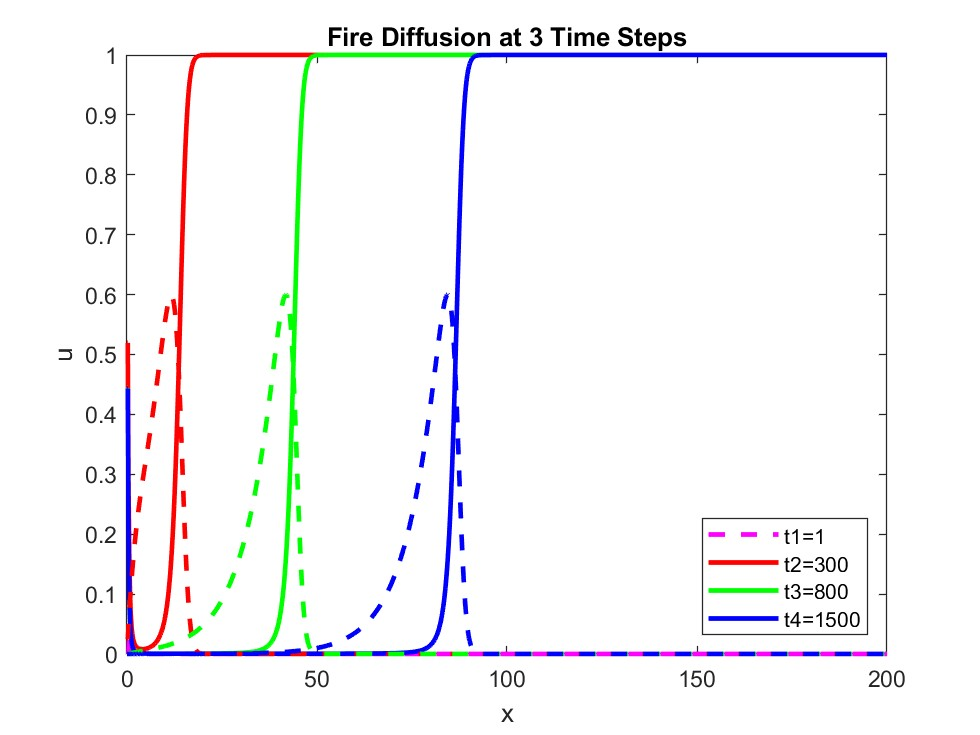
\includegraphics[scale=0.20]{Step1_HS_Gaussian_Advection_Diffusion_3_timestamps.jpg}
    $\textcolor{MidnightBlue}{S_t=}\text{Healthy Trees,}\quad\textcolor{magenta}{b=}\text{Burn Rate,}$\\
    $\textcolor{MidnightBlue}{I_t=}\text{Burning,}\quad\textcolor{orange}{D=}\text{Spread Rate}$
    \end{minipage}
    %
    \hfill
    %
    \begin{minipage}[t]{.49\textwidth}
    \centering Logan Image of SIR model
     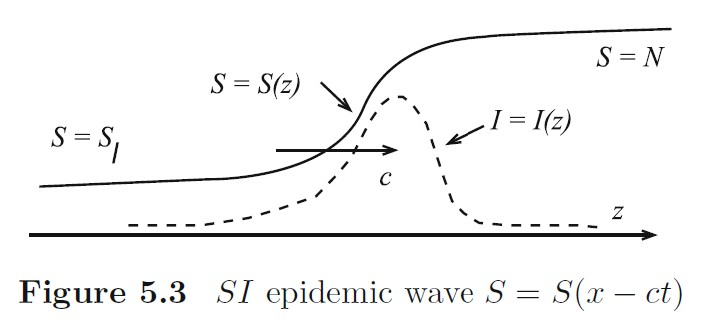
\includegraphics[scale=0.60]{1D_epidemic_from_book.jpg}
     $\textcolor{MidnightBlue}{S_t=}\text{Susceptible,}\quad\textcolor{magenta}{b=}\text{Infection Rate,}$\\
    $\textcolor{MidnightBlue}{I_t=} \text{Infected,}\quad\textcolor{orange}{D=}\text{Diffusion Rate}$
    \end{minipage}

    $D = .5$ Thermal Conductivity/Diffusion coefficient; $b = 1.5$ infection rate of those exposed; $r = .2$  Fatality Rate;  
    $L = 1000$ Total Spatial Length; $J = 5000$ Number Spatial Steps; $h = L/J$ Spatial Step Size; $TT = 100$ Total Time; $N=2000$ Number Time Steps; $k = (h^2)/(D*2)$ Size Time Steps
\vspace{.5cm}    \\
In the graph on the left the solid lines represent the unburned fuel amount at different time steps; $1,300,800,1500$. The dotted lines show the burning region at those same time steps. At a given location all the trees to the right of that location remain healthy until burning begins.  Once the fire front passes all the trees are burned resulting in a $u$ value of $0$ to the left of that location.  The graph on the right is the image from Logan chapter 5.2 that shows a 1D representation of an epidemic wave at an arbitrary time step.  The solid line represents the susceptible population and the dotted line represents those people experiencing infection.  The solid line on the spatial domain does not go to $0$ on the left because not all the people who experience disease in an SI model die or become entirely immune.  At the end of the disease spread process there will be susceptible people.  In fact, if a disease were to result in a $100\%$ fatality rate it is likely it would die out before it could spread.  \\

Studying the forward difference method proved remarkably useful. The above model behavior is better understood having approached them numerically. Being able to manipulate parameters quickly allowed for a deeper understanding of what the math was showing.  
\clearpage    
% ------------- Summary Conclusion
\section{Summary \& Next Steps}
We began this project with the goal of learning about wildfire modeling.  We had not yet intuitively understood how the elements of the SI model contributed to its behavior on the 1D traveling wave graphic in Logan.  We concluded this project with a much deeper understanding not only of the SI model, but a greater appreciation of the utility of numerical methods. We were pleasantly surprised with the relative simplicity of implementing finite difference methods.  We were disappointed that time did not allow us to  implement these techniques in the idealized model.  Next steps in our research would include coding \& analyzing the idealized model and exploring  Diffusion-Reaction type equations like Fisher-KPP below:  
\vspace{1cm}\\
\begin{minipage}[t]{.49\textwidth}
    \centering
    MATLAB Programmed Result
    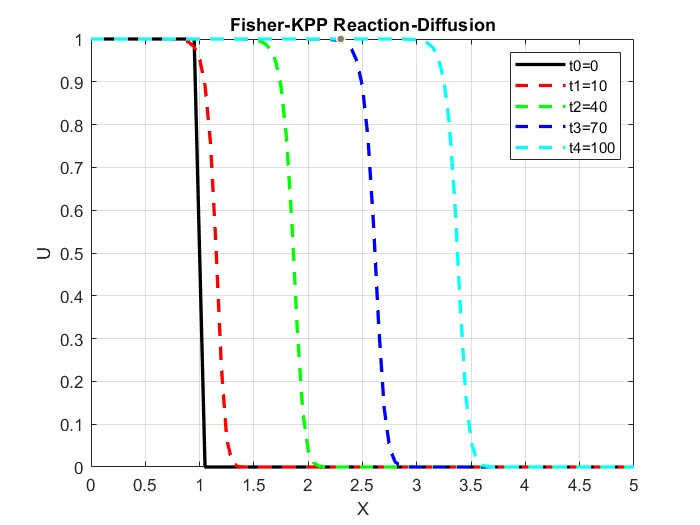
\includegraphics[scale=0.30]{HS_Reaction_Diffusion_5_timestamp.jpg}
    \captionsetup{justification=centering}
    \captionof{figure}{Example of Reacion-Diffusion Equation $\textcolor{MidnightBlue}{u_t} = \textcolor{orange}{D}u_{xx}-\textcolor{red}{ru(1-u)}$}
\end{minipage}
%
\hfill
%
\begin{minipage}[t]{.49\textwidth}
    \centering
    MATLAB Programmed Result
    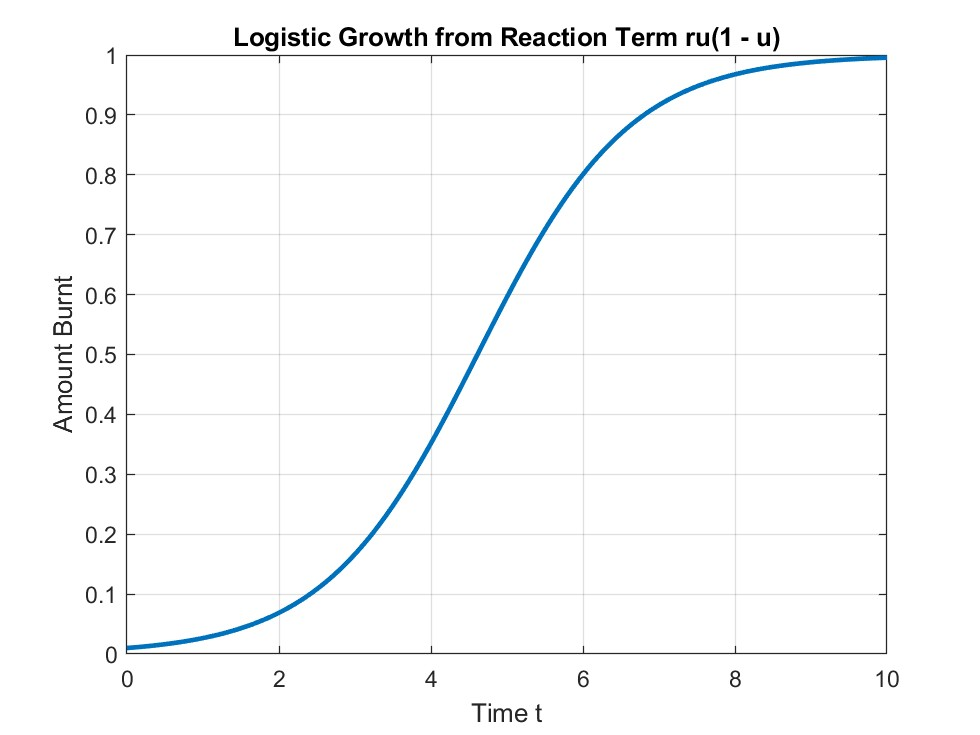
\includegraphics[scale=0.21]{Logistic_image.jpg}
    \captionsetup{justification=centering}
    \captionof{figure}{Logistic Reaction Term \\ $\textcolor{red}{ru(1-u)}$}
\end{minipage}

\vspace{1cm}
We are looking forward to coding the idealized forest fire model as well.  Analyzing these tools, implemented in these models has been a useful area of research and we look forward to using them in our future applied math studies.

%-------------------
\clearpage
\section{Cited Work}
\printbibliography


\end{document}
